\documentclass[hyperref={pdfpagelabels=false},table]{beamer}
\usepackage{../estilo-apresentacao/slides-utfpr}

%\hypersetup{pdfpagemode=FullScreen}   %%% para deixar no modo de tela cheia
\beamertemplatenavigationsymbolsempty   %%% para não mostrar ícones de navegação no canto direito inferior

% Nome da disciplina - informação que somente aparece nas propriedades do arquivo PDF
\subject{Desenvolvimento de Aplicaç\~{o}es Distribu\'{i}das - UTFPR}

\title[Desenv. Apl. Distribu\'{i}das - AD23S - 2018/2]{Desenvolvimento de Aplicaç\~{o}es Distribu\'{i}das}
\subtitle{Aula 5: Comunica\c{c}\~{a}o entre processos remotos/objetos distribuídos}
\author[Prof. Dr. F\'{a}bio Favarim]{Prof. Dr. F\'{a}bio Favarim \texorpdfstring{\\ \footnotesize{favarim@utfpr.edu.br}}{}}
\institute[UTFPR]{ 
\small{\textbf{Universidade Tecnológica Federal do Paraná}}\\
C\^{a}mpus Pato Branco
}


\date{20 de Agosto de 2018}

\begin{document}

\begin{frame}
	\titlepage
\end{frame}

\begin{frame}
	\frametitle{Objetivos da Aula}
	\begin{block}{}
		\begin{itemize}
			\item Entender os princípios da comunicação entre processos remotos 
			\item Sincronização entre processos
			\item Sockets: UDP e TCP
			\item Estudo de Caso:  API Java para Sockets UDP
		\end{itemize}
	\end{block}
	\vspace{2cm}

\end{frame}

\section{Princípios da Comunicação entre processos Remotos}
\subsection{Passagem de Mensagem}

\frame[t]{\frametitle{Princípios da Comunicação Inter-Processos Remotos}
  \begin{block}{Comunicação através da troca de mensagens}
    Toda comunicação entre dois processos remotos somente ocorre através da \alert{\textbf{troca de mensagens via rede}}.        
    A troca de mensagem entre dois pares de processos pode ser implementado por duas operações básicas: send e receive.
    \begin{itemize}
       \item \textbf{send:} processo invoca para enviar mensagem (sequencia de bytes)	
       \item \textbf{receive:} processo invoca para receber mensagem 
    \end{itemize}
  \end{block}
  \begin{block}{Sincronização}
    \begin{itemize}
       \item A comunicação entre dois processos envolve sempre um \alert{mecanismo de sincronização}. 
       \item Envolve saber quando enviar (send) ou receber (receive) dados
       \item Dois tipos: comunicação síncrona x comunicação assíncrona
    \end{itemize}
   \end{block}
}

\subsection{Sincronização}
\frame[t]{\frametitle{Princípios da Comunicação Inter-Processos Remotos}
   \begin{block}{Comunicação Síncrona}
    Transmissor e receptor sincronizam a cada mensagem.
     \begin{itemize}
       \item Envio (send): o processo (ou thread) emissor é bloqueado até que a recepção correspondente seja realizada
       \item Recebimento (receive): o processo (ou thread) receptor fica bloqueado até a recepção correspondente ser realizada   
    \end{itemize}
    Send e Receive são bloqueantes.
   \end{block}

  \begin{block}{Comunicação Assíncrona}
    \begin{itemize}
       \item Envio: o processo envia a mensagem e não fica aguardando após invocar \textbf{send}; 
       \item Recebimento (bloqueante):  o processo fica \textbf{bloqueado} até a recepção ser realizada
       \item Recebimento (não-bloqueante): se não tem nada para receber (na fila), o processo continua seu processamento
     \end{itemize}
   \end{block}
}

\subsection{Endereçamento de Mensagem}
\frame[t]{\frametitle{Princípios da Comunicação Inter-Processos Remotos}
   \begin{block}{Para onde enviar a mensagem???}
    Para saber onde enviar uma mensagem a um processo é preciso saber a localização:
     \begin{itemize}
       \item Endereço IP: permite que a mensagem chegue até o host de destino
       \item Porta: permite que no host a mensagem seja entregue ao processo correto
    \end{itemize}
   \end{block}
}

\subsection{Protocolos}
\frame[t]{\frametitle{Princípios da Comunicação Inter-Processos Remotos}
   Para que dois processos remotos possam se entender, ambos devem usar o mesmo \textbf{protocolo}.

   \begin{block}{Protocolos}
      protocolos definem o \textbf{formato}, \textbf{ordem} das mensagens enviadas e recebidas e \textbf{ações} tomadas no envio ou recepção de mensagens.
   \end{block}
   \begin{figure}
      \centering
      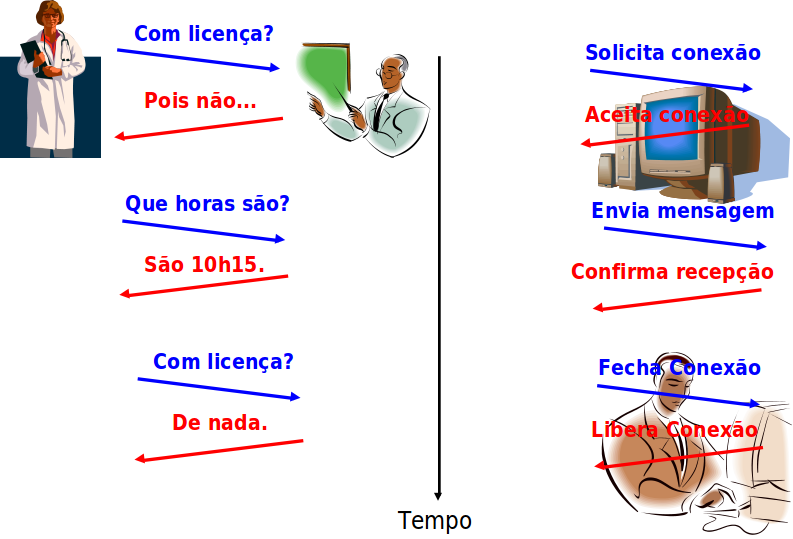
\includegraphics[scale=.25]{figs/protocolo}
    \end{figure}
}


\section{Sockets}
\title[Sistemas Distribu\'{i}dos]{Sockets}
\frame{\titlepage}
\frame[t]{\frametitle{Sockets}
   \begin{block}{Sockets}
     \begin{itemize}
      \item É a interface provida pela camada de transporte para comunicação via rede. 
      \item \textbf{Somente} através de \textbf{\textcolor{blue}{sockets}} é possível enviar uma mensagem via rede.
      \item \textbf{Qualquer tecnologia} que troca mensagens via rede, por baixo \textbf{\textcolor{blue}{sempre}} usa sockets.
      \item API em C criada em 1983 no 4.2 BSD UNIX, é padrão em todos S.O.
     \end{itemize}
   \end{block}
   \begin{figure}
      \centering
      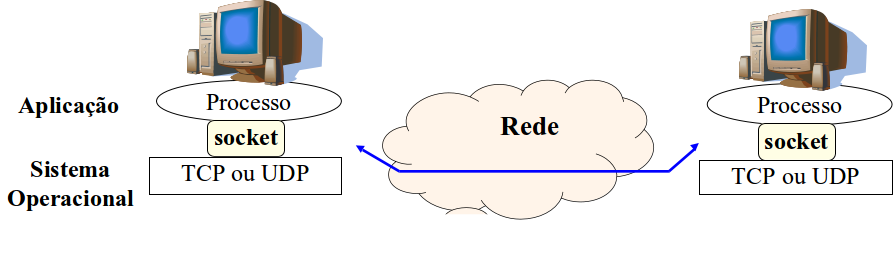
\includegraphics[scale=.35]{figs/sockets}
    \end{figure}
}

\frame[t]{\frametitle{Sockets}
      Os sockets adotam por padrão o paradigma cliente/servidor.
     \begin{itemize}
	\item \textbf{Servidor:} cria o socket em um \textbf{porta conhecida} e fica na escuta a espera de mensagens dos clientes
	\item \textbf{Cliente:} cria o socket em um \textbf{porta qualquer} e envia mensagens através de seu socket para o servidor
     \end{itemize}

   \begin{figure}
      \centering
      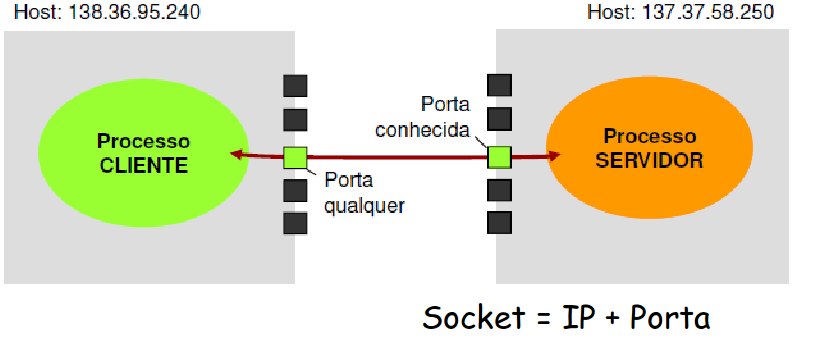
\includegraphics[scale=.35]{figs/sockets-cs}
    \end{figure}
}

\frame[t]{\frametitle{Sockets}
   Um socket é identificado pelo par - \textbf{IP:PORTA}
   \begin{figure}
      \centering
      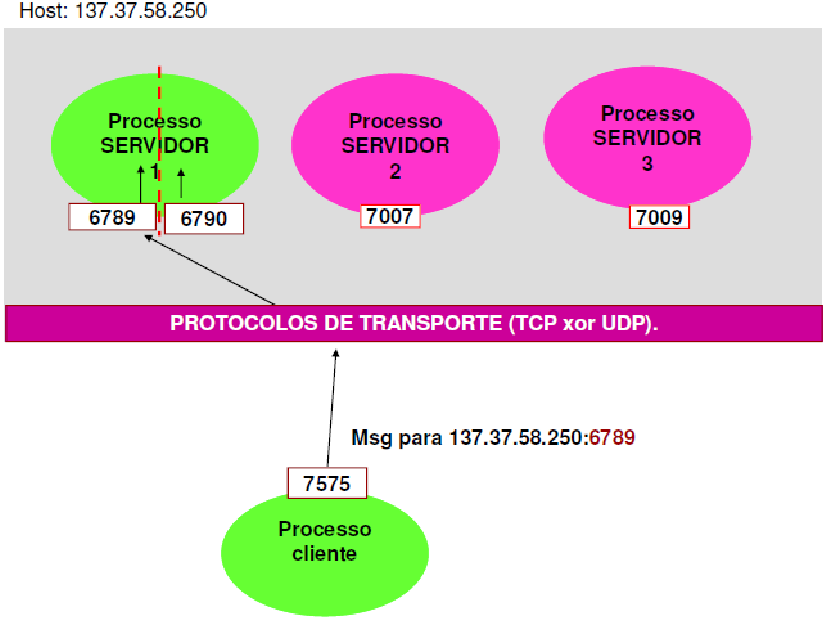
\includegraphics[scale=.32]{figs/sockets-portas}
    \end{figure}
}


 \frame[t]{ \frametitle{Sockets: Modos de Operação}
   \begin{block}{TCP (\textit{Transfer Control Protocol}): Orientado a Conexão}
       \begin{itemize}
        \item As mensagens são enviadas através de um canal de comunicação.
        \item Fluxo contínuo -- são trocadas diversas mensagens consecutivas e estão relacionadas entre si -- ex: vídeo
       \end{itemize}

	  
   \end{block}

   \begin{figure}
     
\includegraphics[scale=.26]{figs/tcp}
   \end{figure}

   \begin{block}{UDP (\textit{User Datagram Protocol}): Não orientado a Conexão}
          \begin{itemize}
           \item Mensagens de tamanho fixo (datagramas) são transmitidas \textbf{individualmente} para destinos especificos.
           \item Cada mensagem é tratada como uma unidade completa de informação
          \end{itemize}
	  
   \end{block}
   \begin{figure}
     
\includegraphics[scale=.26]{figs/udp}
   \end{figure}
}

\subsection{Sockets UDP}
\frame[t]{ \frametitle{Sockets: UDP - User Datagram Protocol}
   \begin{figure}
     
\includegraphics[scale=.26]{figs/udp}
   \end{figure}

   \begin{block}{UDP: Sem conexão – Não confiável}
      \begin{itemize}
	\item Mensagens de tamanho fixo (datagramas) são transmitidas \textbf{individualmente} para destinos especificos.
	\item \textbf{não garante a \alert{entrega}} dos datagramas (\textbf{confiabilidade})
	\item \textbf{não garante a \alert{ordem} da entrega} (\textbf{ordenamento})
	\item endereço destino é especificado em cada datagrama
	\item não há estabelecimento da conexão
	\item \alert{Ex:} Correspondência via serviço postal, VoIP, DNS
      \end{itemize}
   \end{block}
}

\begin{frame}[t]
	\frametitle{Sockets UDP: Sem conexão – Não confiável}
	\begin{itemize}
		\item \textbf{Analogia aos Correios}
		\item Envio de cartas destinadas a um endereço;
		\item O endereço da origem/destinho é adicionado \textbf{a cada carta} enviada;
		\item A maioria das cartas chega mas algumas podem ser perdidas no caminho;
		\item As cartas provavelmente chegarão na ordem em que foram enviadas mas não há garantias;
		\begin{itemize}
			\item Quanto mais distante se estiver do destinatário,maior a probabilidade das cartas chegarem fora de ordem ou serem perdidas;
		\end{itemize}
		\item É possível numerar as cartas e o destinatário lhe escrever solicitando aquelas que não recebeu.
		\end{itemize}
\end{frame}

\subsection{Sockets TCP}
\frame[t]{ \frametitle{Sockets: TCP - Transfer Control Protocol}
   \begin{figure}
     
\includegraphics[scale=.26]{figs/tcp}
   \end{figure}

   \begin{block}{TCP: Orientado a conexão – Confiável}
      \begin{itemize}
	\item Uma conexão deve ser estabelecida antes da transmissão dos dados;
	\item A conexão deve ser encerrada após a transmissão dos dados;
	\item Dados são enviados em fluxo contínuo (stream) na conexão (canal) 
	\item Não são enviados datagrama a datagrama, mas segmentados pelo TCP automaticamente em segmentos
	\begin{itemize}
	  \item Basta gravar no stream para enviar uma mensagem
	  \item Basta ler do stream para receber uma mensagem
        \end{itemize}
	\item É \textbf{garantida \alert{a entrega}} dos segmentos
	\item É \textbf{garantida \alert{a ordem} de entrega} dos segmentos
        \end{itemize}
   \end{block}
}
\begin{frame}[t]
	\frametitle{Sockets TCP: Orientado a conexão – Confiável}
	\begin{itemize}
	 \item \textbf{Analogia ao Sistema Telefônico}
	 \item É necessário discar um número, o outro lado atende e uma \textbf{conexão é estabelecida};
	 \item Cada lado da conversa escuta as palavras na ordem em que foram emitidas (confiabilidade/ordenamento);
	 \item Se não há resposta ou o telefone está ocupado é rapidamente detectado.
	 \item O endereço (número do telefone) do destino somente é preciso ser especificado uma única vez.
	\end{itemize}
\end{frame}


\frame[t]{ \frametitle{Sockets: TCP x UDP}
   \begin{figure}
     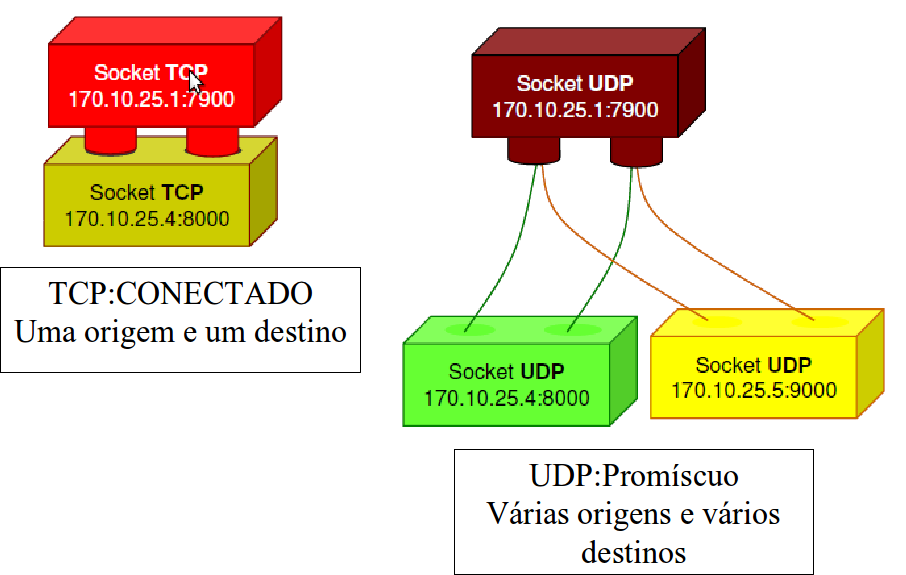
\includegraphics[scale=.33]{figs/sockets-tcpudp}
   \end{figure}
}

\section{Programação com Sockets UDP}
\subsection{Visão Geral}
\begin{frame}[t]
  \frametitle{Passos para comunicação usando Socket UDP}
    \begin{itemize}
     \item Passo 1: criar socket 
	 \item Passos 2/3: realizar a comunicação (enviando e recebendo datagramas usando send e receive)
	 \item Passo 4: fechar socket
    \end{itemize}
% 	\begin{block} {Principais classes Java utilizadas}
% 		\begin{itemize}
% 			\item DatagramSocket
% 			\item DatagramPacket
% 		\end{itemize}
% 		Para enviar dados, insere-se os mesmos em um \textbf{DatagramPacket}, enviando-o através do \textbf{DatagramSocket}.
% 	\end{block}
	\centering
	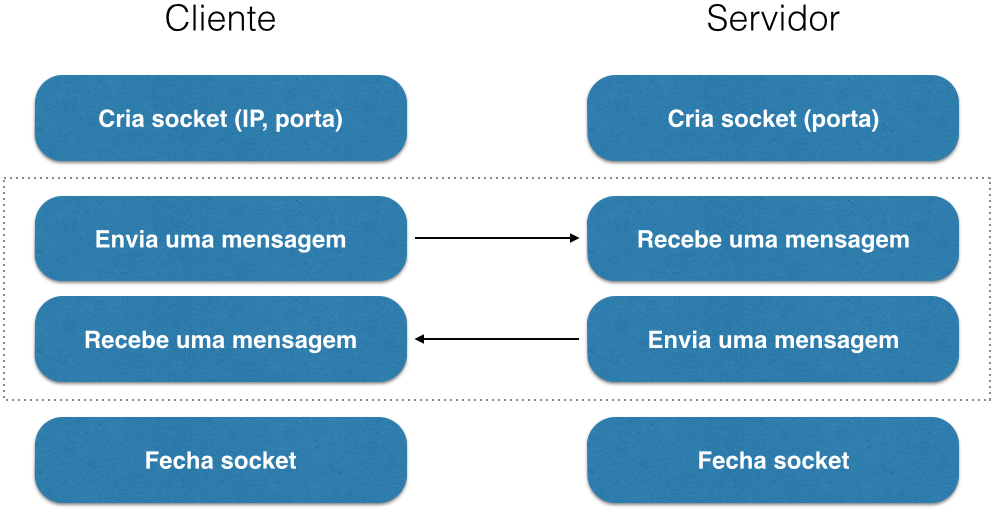
\includegraphics[width=0.85\linewidth]{figs/udp2}

\end{frame}


\subsection{Estudo de Caso - Sockets UDP em Java}
\frame[t]{\frametitle{Programação com Sockets UDP em Java}
  \begin{block}{Pacote \textbf{java.net}, principais classes:}

    \begin{itemize}
      \item \textbf{UDP:} DatagramPacket e DatagramSocket;
      \item Outras: obtenção endereço IP e porta de um pacote, entre outras coisas.
     \end{itemize}
     Para enviar dados, insere-se os mesmos em um \textbf{DatagramPacket}, enviando-o através do \textbf{DatagramSocket}.
  \end{block}
}

% \begin{frame}[t]
%   \frametitle{Passos para comunicação usando Socket UDP}
%     \begin{itemize}
%      \item Passo 1: criar socket em porta especifica.
% 	 \item Passo 2: realizar a comunicação enviando e recebendo datagramas usando send e receive
% 	 \item Passo 3: fechar socket
%     \end{itemize}
% 	\begin{block} {Principais classes Java utilizadas}
% 		\begin{itemize}
% 			\item DatagramSocket
% 			\item DatagramPacket
% 		\end{itemize}
% 		Para enviar dados, insere-se os mesmos em um \textbf{DatagramPacket}, enviando-o através do \textbf{DatagramSocket}.
% 	\end{block}
% 
% \end{frame}

\begin{frame}[t]
\frametitle{Sockets UDP (Java) - Classe DatagramSocket}
	\begin{itemize}
	\item \textbf{DatagramSocket(int port, InetAddress addr)} - cria um socket datagrama, ligado a um endereço local (addr, port) específico.
	\item \textbf{Métodos:}
		\begin{itemize}
			\item \textbf{void receive(DatagramPacket p)}: recebe um pacote de datagrama deste socket.
			\item \textbf{void send(DatagramPacket p)}: envia um pacote de datagrama deste socket.
			\item \textbf{InetAddress getLocalAddress()}: retorna o endereço \textbf{local} do socket
			\item \textbf{int getLocalPort()}: retorna o número de porta \textbf{local} do socket
			\item \textbf{void close()}: fecha o socket deste datagrama.
		\end{itemize}
	\end{itemize}
\end{frame}

\begin{frame}[t]
	\frametitle{Sockets UDP (Java) - classe DatagramPacket}
	\begin{itemize}
		\item \textbf{DatagramPacket(byte[] dados, int tamanho, InetAddress endereco, int porta)}: constrói um datagrama para \alert{enviar} \textbf{dados} de \textbf{tamanho} para uma máquina em um \textbf{endereço} e \textbf{porta} específicos.
		\item \textbf{DatagramPacket(byte[] buf, int tamanho)}: constrói um datagrama para \alert{receber} \textbf{dados} com determinado \textbf{tamanho}.
 		\item \textbf{Métodos:}
		\begin{itemize}
			\item \textbf{InetAddress getAddress()}: retorna o endereço da origem do datagrama;
			\item \textbf{int getPort()}: retorna o número de porta da origem do datagrama;
			\item \textbf{byte[] getData()}: retorna os dados contidos no datagrama;
			\item \textbf{int getLength()}: retorna o tamanho dos dados do datagrama.
		\end{itemize}
	\end{itemize}
\end{frame}

\begin{frame}[fragile]
\frametitle{Sockets UDP (Java) - Comandos Básicos}

Criar Socket
\begin{lstlisting}
    DatagramSocket socket = new DatagramSocket(porta);
\end{lstlisting} 

Fechar Socket
\begin{lstlisting}
    socket.close();
\end{lstlisting} 

Enviar Datagrama
\begin{lstlisting}
    socket.send(dgEnvio);
\end{lstlisting} 

Receber Datagrama
\begin{lstlisting}
    socket.receive(dgRec);
\end{lstlisting} 
\end{frame}

\begin{frame}[fragile]
	\frametitle{Sockets UDP (Java) - Comandos Básicos}

	Criar um datagrama para enviar dados
	\begin{lstlisting}
    	dgEnvio = new DatagramPacket(msg, msg.length, endereco, porta);
	\end{lstlisting} 

	Criar um datagrama para receber dados
	\begin{lstlisting}
		dgRec = new DatagramPacket(buffer, buffer.length);
	\end{lstlisting} 

	\alert{Importante}
		\begin{lstlisting}
			endereco = InetAddress.getByName(``172.29.100.100'')
			msg e buffer = array de bytes(byte[])
		\end{lstlisting} 

	\alert{Comando Extras}
		\begin{lstlisting}
			datagrama.getAddress();	//obtem IP de origem
			datagrama.getPort());    //obtem porta de origem
		\end{lstlisting} 

\end{frame}


\begin{frame}[fragile]
	\frametitle{Sockets UDP (Java) - Programa Cliente}

	\begin{lstlisting}
		//Dados do servidor
		InetAddress endereco = InetAddress.getByName("127.0.0.1");
		int porta = 4321;

		//Passo 1: criar socket
		DatagramSocket socket = new DatagramSocket();
		
		//Passo 2: realizar a comunicacao com o servidor (ficar em loop???)
		String mensagem = "Alo galera maneira";
		byte[] msg = mensagem.getBytes();
		DatagramPacket dgEnvio= new DatagramPacket(msg,msg.length,endereco,porta);
		socket.send(dgEnvio);

		//recebimento dos dados do servidor - fica bloqueado no receive
		DatagramPacket dgRec = new DatagramPacket(new byte[1024],1024);
		socket.receive(dgRec); 

		String msgRecebida = new String(dgRec.getData());

		//Passo 3: fecha socket
		socket.close();
	\end{lstlisting} 

\end{frame}

\begin{frame}[fragile]
	\frametitle{Sockets UDP (Java) - Programa Servidor}

	\begin{lstlisting}
		//Passo 1: criar socket em porta especifica.
		DatagramSocket socket = new DatagramSocket(4321);

		//Passo 2: realizar a comunicacao com o cliente (ficar em loop??)
		// cria datagrama para receber requisicao do cliente
		DatagramPacket dgRec = new DatagramPacket(new byte[1024], 1024);
		socket.receive(dgRec);

		String mensagem = new String(dgRec.getData()).trim();
		System.out.println("Recebeu " + mensagem + " de "+ 
		                        dgRec.getAddress() + ":" + dgRec.getPort());
		
		// envia resposta
		DatagramPacket dgEnvio = new DatagramPacket(dgRec.getData(), gdRec.getLength(),
		dgRec.getAddress(), dgRec.getPort());
		socket.send(dgEnvio);

		// Passo 3: fecha o socket (somente quando terminar o servidor)
		socket.close();	
\end{lstlisting} 

\end{frame}
\frame[t]{ \frametitle{Exercícios}
	 \begin{itemize}
		\item Resolução da Prática 2 (exercícios UDP)
		\item Códigos apresentados nos slides estão disponíveis no Moodle
		\item Agora: Alo mundo com Sockets UDP!!! 
	 \end{itemize}
}

\frame[t]{ \frametitle{Próxima aula}
	 \begin{itemize}
	  \item Estudo de Caso: Sockets UDP em C
	 \end{itemize}
}
\end{document}
